\documentclass[10pt,a4paper]{article}
\usepackage[T1]{fontenc}
\usepackage{lmodern}
\usepackage[margin=2.1cm]{geometry}
\usepackage{microtype}
\usepackage{amsmath}
\usepackage{booktabs,tabularx,longtable}
\usepackage{enumitem}
\usepackage[dvipsnames]{xcolor}
\usepackage{tikz}
\usetikzlibrary{arrows.meta,positioning}
\usepackage{titlesec}
\usepackage[colorlinks=true,linkcolor=MidnightBlue,urlcolor=MidnightBlue]{hyperref}
\setlist{itemsep=2pt,topsep=3pt}
\titleformat{\section}{\large\bfseries\color{MidnightBlue}}{\thesection}{0.6em}{}
\titleformat{\subsection}{\normalsize\bfseries}{\thesubsection}{0.6em}{}
\newcommand{\code}[1]{\texttt{\small #1}}
\newcolumntype{L}{>{\raggedright\arraybackslash}X}
\newcommand{\status}[1]{\textsf{\footnotesize\bfseries #1}}

\title{\textbf{MORPHOS v2}\\[2pt]\large Sharp, vibrant reaction--diffusion as the instrument\\[2pt]\normalsize Design document \textperiodcentered{} branch \code{morphos-v2}}
\author{IAmM3ta/morphogen}
\date{October 2026}

\begin{document}
\maketitle

\begin{center}\fbox{\parbox{0.92\linewidth}{\small
\textbf{Priority (top of the build order).} v2 is a seamless, synesthetic convergence of
\emph{sharp} (high resolution, crisp, never blurred) and \emph{vibrant, psychedelic}
reaction--diffusion. The Gray--Scott field \emph{is} the main visual. Sound drives the
chemistry itself (feed/kill, diffusion ratio, anisotropy, onset seeding, palette); tilt and
compass steer anisotropy and flow. A WebGPU compute port is the primary path; the existing
WebGL2 field is strictly the fallback when \code{navigator.gpu} is absent or fails. Looks are
colourings, lighting and optional kaleidoscopic symmetry of the simulated domain. Adaptive
quality lowers the step count, then the simulation grid, and never the output resolution.}}\end{center}

\tableofcontents

%======================================================================
\section{Sharp RD convergence (the core)}

\subsection{Reference: Karl Sims' RD Tool}
The visual target is Karl Sims' reaction--diffusion work: the tutorial
(\href{https://www.karlsims.com/rd.html}{karlsims.com/rd.html}) and the RD Tool
(\href{https://www.karlsims.com/rdtool.html}{karlsims.com/rdtool.html}, help page
\href{https://www.karlsims.com/rdtool-help.html}{rdtool-help.html}). We read both. What we took from them:

\begin{itemize}
\item \textbf{Model.} Gray--Scott with $D_A=1$, $D_B=0.5$, $f=0.055$, $k=0.062$, $\Delta t=1$:
\[
A' = A + (D_A\nabla^2 A - AB^2 + f(1-A))\Delta t,\qquad
B' = B + (D_B\nabla^2 B + AB^2 - (k+f)B)\Delta t .
\]
\item \textbf{Laplacian.} 3$\times$3 convolution: centre $-1$, adjacent $0.2$, diagonals $0.05$.
We use exactly this stencil.
\item \textbf{Regimes.} The tutorial gives mitosis at $f=0.0367,k=0.0649$ and coral at
$f=0.0545,k=0.062$. The pattern map spans $k\in[0.045,0.07]$ and $f\in[0.01,0.1]$.
\item \textbf{Options the RD Tool exposes.} \emph{Orientation} (anisotropic diffusion),
\emph{Style map} (feed/kill varying across the grid: radial, ring, random, horizontal, vertical),
\emph{Flow} (a velocity field that advects the chemicals), \emph{Scale} (reaction rate vs.\ diffusion
rate), brush seeding, 12 colour maps with emboss and invert, and colour controls (hue, saturation,
brightness, contrast, frequency, phase).
\item \textbf{Look.} The videos use embossed height-map lighting on $B$, with crisp edges at high
resolution. The RD Tool runs on WebGL2 + \code{EXT\_color\_buffer\_float} + WASM. We do the same
job as WGSL compute on WebGPU.
\end{itemize}

\subsection{What ``sharp'' means here}
\begin{enumerate}
\item \textbf{The grid follows device pixels.} The long side is $\min(\text{cap},\ \text{css}\times\text{dpr})\times\text{scale}$.
The cap is 2048 on desktop and 1600 on coarse-pointer devices. The DPR cap defaults to 3 (2 in wallpaper mode).
\item \textbf{Many steps per frame}: 6--40, governed (Section~\ref{sec:gov}).
\item \textbf{Crisp render.} The colour index uses a threshold with derivative anti-aliasing,
$\mathrm{smoothstep}(t-a,t+a,B)$ where $a=\max(1.1\,\mathrm{fwidth}(B),\,0.0012)$. Edges are therefore
one output pixel wide at any zoom, never a blur kernel.
\item \textbf{Lighting comes from exact texel gradients.} The emboss normal is built from one-texel central
differences of $B$. Specular and Fresnel terms give the gold and chrome looks.
\item \textbf{No resampled output.} The final pass reads the scene with \code{textureLoad} at the exact pixel.
Bloom is a separate half-resolution layer that is \emph{added}, so it never replaces detail.
\item \textbf{Quality never blurs.} The governor lowers steps first, then the sim grid. The canvas
always matches device pixels (up to the DPR cap).
\end{enumerate}

\subsection{Audio drives the chemistry}
All features are smoothed with asymmetric attack and release before they touch the solver.
$k_r$ is the user's \emph{Reactivity} (0--2).

\begin{center}\small
\begin{tabularx}{\linewidth}{@{}l L L@{}}
\toprule
Feature & RD parameter & Mapping (as implemented)\\
\midrule
Bass (sub+bass) & feed $f$, swirl, bloom knee & $f \mathrel{+}= 0.0045\,\bar b\,k_r$; swirl $\times(0.6+0.6\bar b)$; bloom threshold $-0.08\,b$\\
Spectral centroid & kill $k$, palette & $k \mathrel{+}= 0.0035(\bar c-0.4)k_r$; hue rotation and accent phase in the scene pass\\
Highs & diffusion ratio & $D_A \times (1+0.08\,\bar h\,k_r)$ (on top of the v1 high-band term)\\
Onsets & local seeding & a new onset ripple plants $B$ at its point, folded $n$-fold for mandala looks. Onsets under a finger and touch-down ripples do \emph{not} seed\\
Drone pitch & fold order & order $=\mathrm{round}(\text{foldBase}-2+6\,\text{pitch}_{\text{norm}})\in[3,12]$, changed only after the pitch holds\\
Spectrum peaks & Chladni style map & $n,m$ of the Cymatic style map follow the dominant bands\\
RMS & bloom, haze & final pass gain\\
\bottomrule
\end{tabularx}\end{center}

\subsection{Sensors steer anisotropy and flow}
\begin{center}\small
\begin{tabularx}{\linewidth}{@{}l L@{}}
\toprule
Input & Effect\\
\midrule
Tilt (x,y) & Direction of anisotropic diffusion ($\theta=\mathrm{atan2}(t_y,t_x)$). Strength $+\min(0.3,0.45|t|)k_r$, capped at 0.6. Flow velocity $+0.35\,t\,k_r$\\
Compass heading & Orientation angle when the device is flat; v1 heading$\to$scale is kept\\
Neither & Slow orientation drift, so the field never freezes in one direction\\
Desktop & Wheel, Shift+wheel and the arrow keys emulate tilt and compass (\code{bindDesktopControls})\\
\bottomrule
\end{tabularx}\end{center}
Stability: the anisotropic term $a\cdot\tfrac12(\partial_{dd}-\partial_{pp})$ is added to the 9-point
Laplacian, and $D\,\Delta t$ is clamped to $1.8/(1.6+2a)$.

\subsection{Regimes morph}
\code{RegimeDrift} holds a regime, then glides feed and kill to the next:
spots (0.0353, 0.0653), mitosis (0.0367, 0.0649), stripes (0.026, 0.061), labyrinth
(0.029, 0.057), coral (0.0545, 0.062), worms (0.046, 0.063), holes (0.039, 0.058), waves
(0.018, 0.051). The style map blends a second regime spatially (radial, ring, noise,
vertical, Chladni), so two pattern families coexist and their border moves.

%======================================================================
\section{Build order}
\begin{center}\small
\begin{tabularx}{\linewidth}{@{}c l L l@{}}
\toprule
\# & Phase & Content & Status\\
\midrule
1 & WebGPU RD core & WGSL compute Gray--Scott, 9-point + anisotropic Laplacian, style map, flow, seeding, pack, stats & \status{shipped}\\
2 & Crisp render & Scene pass (AA threshold, emboss, specular, LUT, kaleido), bloom, final & \status{shipped}\\
3 & Audio$\to$RD & Features bus $\to$ feed/kill/diffusion/aniso/seeding/palette & \status{shipped}\\
4 & Sensors$\to$RD & Tilt/compass $\to$ anisotropy and flow & \status{shipped (untested on device)}\\
5 & Looks & Eight RD colourings with lighting and symmetry & \status{shipped}\\
6 & Governor & Steps$\to$grid ladder, GPU backpressure & \status{shipped}\\
7 & Fallback & WebGL2 RDEngine + palette-only looks; device-loss failover & \status{shipped}\\
8 & Sound engine v2 & Drone, bass, drums, transport, loop, WAV & \status{shipped}\\
9 & v2 UI & Dock, panels, glass, fullscreen, keys & \status{shipped}\\
10 & Wallpaper + PWA & \code{/wallpaper}, URL options, manifest & \status{shipped}\\
11 & Docs & README, CHANGELOG, this document & \status{shipped}\\
12 & Video-informed looks & Lighting pass, ripple layer, bloom chain, Iridescent, Oscillators, Hex Cymatic, Fluidica & \status{shipped (headless-verified)}\\
\bottomrule
\end{tabularx}\end{center}

%======================================================================
\section{WebGPU architecture}

\subsection{Passes}
\begin{center}
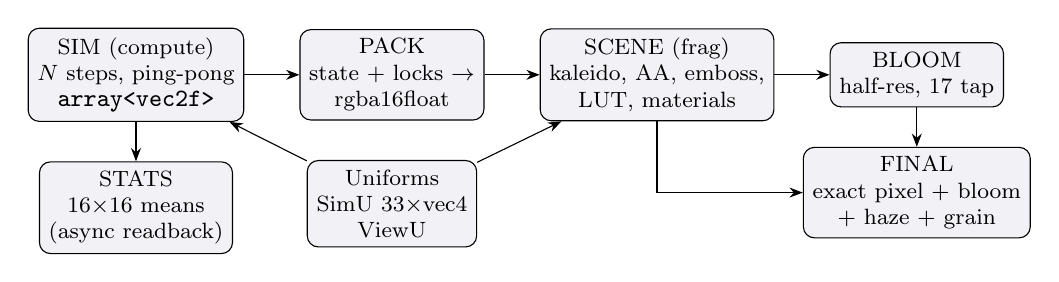
\begin{tikzpicture}[node distance=5mm and 7mm, box/.style={draw,rounded corners,align=center,font=\footnotesize,minimum height=8mm,fill=MidnightBlue!6}, >=Stealth]
\node[box] (sim) {SIM (compute)\\$N$ steps, ping-pong\\\code{array<vec2f>}};
\node[box,right=of sim] (pack) {PACK\\state + locks $\to$\\rgba16float};
\node[box,right=of pack] (scene) {SCENE (frag)\\kaleido, AA, emboss,\\LUT, materials};
\node[box,right=of scene] (bloom) {BLOOM\\half-res, 17 tap};
\node[box,below=of bloom] (final) {FINAL\\exact pixel + bloom\\+ haze + grain};
\node[box,below=of sim] (stats) {STATS\\16$\times$16 means\\(async readback)};
\node[box,below=of pack] (uni) {Uniforms\\SimU 33$\times$vec4\\ViewU};
\draw[->] (sim)--(pack); \draw[->] (pack)--(scene); \draw[->] (scene)--(bloom); \draw[->] (bloom)--(final);
\draw[->] (scene.south) |- (final.west);
\draw[->] (sim)--(stats); \draw[->] (uni)--(sim); \draw[->] (uni)--(scene);
\end{tikzpicture}
\end{center}

\begin{itemize}
\item \textbf{SIM}: a 16$\times$16 workgroup. Per cell: the 9-point Laplacian plus the anisotropic term.
Semi-Lagrangian bilinear advection runs only when $|v|>0.02$. The style map blends $f,k$ with a second regime. Brushes, the finger wake,
beat seeding, onset seeds folded $n$-fold, MorphoMark lock planting, image modes, and noise are all handled here.
\item \textbf{PACK}: writes $(A,B,\text{lockGhost})$ to an \code{rgba16float} storage texture, flipped so row 0 is the top.
\item \textbf{SCENE}: folds the domain into a kaleidoscope (mandala core with a feathered radius, or the full field). It then
applies the AA threshold, emboss normal, specular, thread and iso lines, and per-material shading (Section~\ref{sec:looks}), followed by
the MorphoMark ghosts, soft contour ripples for onsets (never a flash), and the play hue rotation.
\item \textbf{BLOOM / FINAL}: half-resolution bright-pass bloom, then the exact-pixel composite with haze, vignette, soft clip, and grain.
\item \textbf{RESAMPLE}: bilinear state transfer when the sim grid changes size, so the pattern survives the change.
\item \textbf{Capture}: \code{capturePng} renders the full chain offscreen at 2048--3200\,px.
\end{itemize}

\subsection{Robustness}
\begin{itemize}
\item \code{RDGpuEngine.create()} returns \code{\{ok:false, reason\}} instead of throwing. Failure cases: a 4\,s adapter timeout,
WGSL compilation info errors, and a pipeline error scope.
\item Uncaptured errors and device loss call \code{onLost}. The app marks WebGPU as failed for the session
(\code{sessionStorage}), tears down, starts the WebGL2 field, and keeps playing. \code{?gpu=1} retries WebGPU.
\item \textbf{Backpressure.} At most two frames are in flight (\code{onSubmittedWorkDone}). Over that, the
frame is skipped but audio and UI keep ticking. The governor uses $\max(\text{rAF}\ \Delta t, \text{GPU time})$.
\item \textbf{Auto layouts.} Every declared binding is statically used, so \code{layout:"auto"} keeps all of them. One defect of this
kind was found and fixed during smoke testing (the bloom pass did not read its uniform).
\end{itemize}

%======================================================================
\section{Adaptive quality: steps before scale, never blur}\label{sec:gov}
\begin{itemize}
\item Shedding order: steps to 16 $\to$ bloom passes $\to$ ripple grid $\to$ steps to 6 $\to$ sim grid (Section~\ref{sec:video}).
\item Step ladder: 6, 8, 10, 12, 16, 20, 24, 28, 32, 36, 40. The default cap is 32 on desktop and 20 on coarse devices.
\item Grid ladder: $\times$1, 0.85, 0.72, 0.6, 0.5. It is only touched once steps are already at the bottom.
\item The EMA of frame time is compared with the budget ($1000/\text{fps cap}$, or 16.7\,ms). Above $1.22\times$ the budget, step down
(cool-down 90 frames). Below $0.82\times$, recover: grid first, once steps are $\ge16$, then steps (cool-down 240).
\item \code{quality=low} starts at 12 steps and grid $\times$0.6. \code{high} disables the governor.
\item The output canvas is never downscaled. Reduced motion slows simulated time ($\times0.4$) and calms flow and swirl.
\item rAF stops when the tab is hidden. Wallpaper mode defaults to 30\,fps and DPR 2.
\end{itemize}

%======================================================================
\section{Looks: colourings of the field}\label{sec:looks}
Twelve looks: the eight below plus four video-informed looks (Section~\ref{sec:video}).
Each look sets a 256$\times$2 LUT: row 0 is the main map, with frequency and mirror baked in, and row 1 is an accent map. It also sets the lighting,
thread lines, style map, anisotropy, swirl and symmetry. The palettes follow the MEMETiC brief: gold and bronze filigree,
liquid rainbow chrome, teal beams and haze, UV magenta and violet, iridescent accents. There is no face rendering.

\begin{center}\small
\begin{tabularx}{\linewidth}{@{}l L l l l@{}}
\toprule
Look & Character & Kaleido & Style map & Light\\
\midrule
Field & species palette, sharpened (v1 continuity) & none & none & emboss 0.35\\
Marble & silver veins, ink flow; iso lines & none & noise & emboss 0.45\\
Temple Gold & embossed gold filigree, iridescent mandala core, moir\'e halo & core, 8-fold & radial & emboss 1.0, spec 0.85\\
Chrome Bloom & liquid rainbow metal: normal-driven reflection LUT, Fresnel, dark mirror ground & none & noise & emboss 0.9, spec 1.0\\
Teal Beam & light shafts through the growth, cyan threads & none & vertical & emboss 0.3\\
UV Mandala & violet stage, iridescent threads, moir\'e, centre glow & full, 6-fold & ring & emboss 0.5\\
Projection & edge-to-edge cyclic LUT flow, strong swirl & none & noise & emboss 0.4\\
Cymatic & the sound's standing waves (Chladni $n,m$) steer growth & none & Chladni & emboss 0.6\\
\bottomrule
\end{tabularx}\end{center}
On the WebGL2 fallback, a look maps to a four-stop palette (\code{fourStops}) through \code{runtime.v2Stops}. The fallback gets
colour only; it has no kaleidoscope or materials.

%======================================================================
\section{Video-informed looks}\label{sec:video}
Four looks come from an analysis of Metta's inspiration videos (\code{m3metic/video-findings.md}). All four are rendered on the WebGPU path only.
They keep the reaction--diffusion field as the subject and add three things: a lighting pass, a ripple layer, and a three-level bloom chain.

\subsection{Lighting pass (WGSL, materials 8--11)}
\begin{itemize}
\item \textbf{Height and normal}: one-texel central differences of $B$ (emboss gain per look), plus the ripple-layer gradient $\nabla h$.
Optional fine normal noise gives a velvet surface.
\item \textbf{Thin film}: a Schlick Fresnel term $F=F_0+(1-F_0)(1-N\!\cdot\!V)^5$, with the accent LUT (cyan$\to$magenta$\to$gold) indexed by $1-N\!\cdot\!V$,
by $B$, and by a slow phase driven by centroid and time.
\item \textbf{Specular}: GGX (Trowbridge--Reitz) with Schlick--Smith visibility. A warm key light (steered by tilt) and a cool fill each have their own intensity and colour.
\item \textbf{Matte}: wrap diffuse $(N\!\cdot\!L+w)/(1+w)$. Cavity AO compares $B$ with a 4-tap ring mean at 3 texels. Faux SSS adds warmth on the peaks.
\item \textbf{HDR emissive}: lines, webs and contours exceed 1.0 in the \code{rgba16float} scene, feeding the bloom chain. Each look sets its own bright-pass threshold.
\item \textbf{Bloom chain}: a $\tfrac12$-resolution bright pass, then $\tfrac14$ and $\tfrac18$ tent down-samples, combined with per-look weights in the exact-pixel final pass.
\end{itemize}

\subsection{Ripple layer}
\begin{itemize}
\item A low-resolution 2D wave equation with ping-pong buffers, $h' = (2h - h_{-1} + c^2\nabla^2 h)\,d$. Constants: $c^2=0.22$, $d=0.996$, 3 substeps a frame, and damped edges.
The grid is 320 cells on the long side, stepping down to 224 and then 160 under load.
\item \textbf{Impulses}: strong onsets (flux or bass over threshold) drop a Gaussian kick at the centre. Every touch, kick or onset ripple drops a small one where it lands.
\item \textbf{Coupling}: $\nabla h$ refracts the field's sampling UVs in the scene pass. In the sim, crests raise feed ($f \mathrel{+}= g_f h$) and steep fronts raise kill
($k \mathrel{+}= g_k|\nabla h|$), so the ripples reshape the pattern itself.
\end{itemize}

\subsection{The four looks}
\begin{center}\small
\begin{tabularx}{\linewidth}{@{}l L L@{}}
\toprule
Look & From the video & Implementation\\
\midrule
Iridescent & inky navy, thin-film cyan/magenta/gold, hyper-glossy, slow viscous flow, topographic contours & navy LUT; film ramp by Fresnel; GGX roughness 0.18; warm key and cyan fill; glowing iso contours; labyrinth pull 0.45; solver speed $\times0.6$; high bloom threshold\\
Oscillators & dense papillae on rolling waves, slate-teal valleys to peach/gold peaks, velvety, AO, warm tips & mitosis pull 0.9 at $\times0.8$ scale (dense spots); height = $B$ + rolling macro wave; palette mix(slate, peach, smoothstep($h$)); wrap 0.6; cavity AO; faux SSS; normal noise; breathing UV warp\\
Hex Cymatic & glowing amber hex/triangle grid over dark gloss; central cymatic web; ripples from the centre on transients & analytic, \code{fwidth}-anti-aliased hex and triangle lines refracted by $\nabla h$; Chladni-style $\sin(nx)\sin(my)$ / $\cos$ mode pairs plus a radial mode, weighted by the bass, mid and high bands, with order ``tightened'' by centroid; HDR amber emissive\\
Fluidica & \#080C16 liquid, silver highlights \#8B9DB6, a gold grid \#FFF0B3$\to$\#D96600 shattered by one big impact into a branching web & the sim pins a diamond lattice (refracted by the ripples). A bass drop, kick or touch releases it (big central impulse) into a coral-regime web, and it re-forms after 30\,s. Silver Schlick environment term, gold emissive web\\
\bottomrule
\end{tabularx}\end{center}

\subsection{Quality and limits}
Under load, the governor sheds work in this order: steps down to 16, then bloom passes (3$\to$1), then ripple grid (320$\to$160), then steps down to 6, then the sim grid.
Output resolution is never lowered. Depth of field and tilt-shift from the videos are \emph{not} implemented, because they would blur the field, which goes against the
sharpness priority. The low oblique ``camera'' and the melting-cube geometry are also out of scope: the field stays a flat, full-frame surface. The WebGL2 fallback shows these looks as four-stop colourings only.
The same pass fixed a bug: iso lines on the empty ground (where $B\approx0$) caused speckle in Marble.

%======================================================================
\section{Signal flow}
\begin{center}
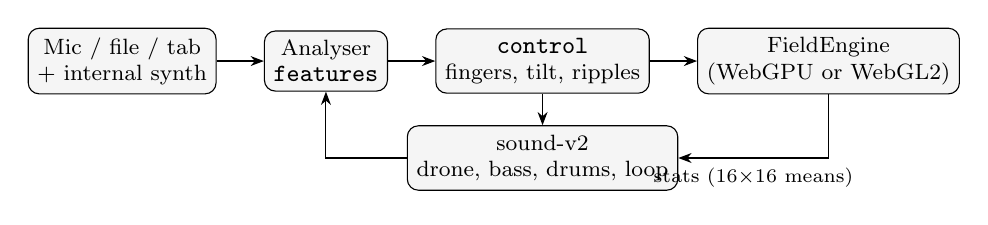
\begin{tikzpicture}[node distance=4mm and 6mm, box/.style={draw,rounded corners,align=center,font=\footnotesize,minimum height=7mm,fill=gray!8}, >=Stealth]
\node[box] (in) {Mic / file / tab\\+ internal synth};
\node[box,right=of in] (an) {Analyser\\\code{features}};
\node[box,right=of an] (ctl) {\code{control}\\fingers, tilt, ripples};
\node[box,right=of ctl] (eng) {FieldEngine\\(WebGPU or WebGL2)};
\node[box,below=of ctl] (snd) {sound-v2\\drone, bass, drums, loop};
\draw[->] (in)--(an); \draw[->] (an)--(ctl); \draw[->] (ctl)--(eng); \draw[->] (ctl)--(snd); \draw[->] (snd.west) -| (an.south);
\draw[->] (eng.south) |- node[pos=0.75,below,font=\scriptsize]{stats (16$\times$16 means)} (snd.east);
\end{tikzpicture}
\end{center}
Per frame, the engine's \code{onFrame} runs the v2 tick first (\code{tickFeatures} $\to$ analyser $\to$ \code{updateControl} $\to$ \code{sound.frame}),
then the unchanged v1 per-frame work (Hum, theremin, Sync TD WS/MIDI, recording).

%======================================================================
\section{Sound engine v2 (summary)}
Drone synth (voices, Hold, in-key or free), a refined 16-step bass with finger record, a four-lane drum machine with mute and solo, a swing transport
with tap tempo, scenes A--D with copy, clear and undo, a drone lane with arm, overdub and bars, a Starter loop, and Export WAV. The output passes through a limiter
and soft clip. Additive hooks on \code{audio-engine.ts} keep The Hum, theremin, Freeze/Release, Rec/Loop and Sync unchanged.

%======================================================================
\section{UI, accessibility and invariants}
\begin{itemize}
\item The mode dock has Field, Drone, Bass, Loop and Look. The top bar gains Full, Glass and Keys. The shortcuts sheet opens with \code{?}.
\item Keys: M (mode), V/Shift+V (look), P (loop), G (glass), F (fullscreen), Esc (close). Keys are disabled in wallpaper mode.
\item Locked copy is unchanged: ``Tap to start sound. Drag to plant growth. Touch the field to hear it.'' and
``Freeze: stop growth. Release: let it grow again.'' Schumann does not appear on the splash, meta or first screen.
\item Enter never requests MIDI (verified headless). Icon-only controls carry \code{aria-label} and \code{title}. There is no double-tap copy or gesture.
\item iOS motion permission and audio unlock happen only inside a user gesture; denial is graceful.
\item Fullscreen uses the standard API with a webkit fallback. Where unavailable (iPhone Safari), the app shows Share $\to$ Add to Home Screen guidance.
\end{itemize}

%======================================================================
\section{Wallpaper mode and PWA}
\code{/wallpaper} or \code{?wallpaper=1} gives no gate, no UI, no prompts, no sensors and no MIDI, and the cursor hides when idle.
Options: \code{visual} (default \code{temple-gold}), \code{quality}, \code{fps} (default 30, 0 means uncapped), \code{dpr} (default 2),
and \code{audio=1} (ambient held drone, where the host allows autoplay).
The manifest adds \code{display\_override: [fullscreen, standalone]}, 192 and 512 icons, and a Wallpaper shortcut.

Hosts. These facts come from the hosts' public documentation only, and MORPHOS has not been tested on any of them:
\begin{itemize}
\item \textbf{Lively Wallpaper (Windows)}: Add wallpaper $\to$ Enter URL. Web wallpapers render in WebView2 (Edge) or CefSharp. Autoplay is
allowed. Lively pauses playback for fullscreen apps and can pause on battery. A packaged Lively wallpaper can receive system audio
through \code{livelyAudioListener} (128 bins) when \code{LivelyInfo.json} has \code{--audio}. That bridge is \emph{not} implemented.
\item \textbf{Plash (macOS)}: add the URL as a website. Audio is muted, it can deactivate on battery, and it injects the class \code{is-plash-app}.
\item \textbf{Android}: third-party ``website as live wallpaper'' apps exist on Google Play. WebGPU inside their WebViews is unverified,
so expect the WebGL2 field. The PWA plus the \code{/wallpaper} shortcut is the first-party route.
\end{itemize}

%======================================================================
\section{Shipped vs.\ designed-but-pending}
\textbf{Shipped:} everything in the build-order table.

\noindent\textbf{Pending or changed:}
\begin{itemize}
\item The Tesseract look was dropped. The particle and beam overlay compositor was dropped in favour of driving the RD field directly.
\item MorphoMark lock ghosts on the WebGPU path use the current LUT. Per-lock palettes are not preserved there.
\item The finger wake (drag advection) is gentler than v1 on the GPU path.
\item The WebGL2 fallback gets palette-only looks.
\item The Lively system-audio bridge and Plash auto-detection are not implemented.
\item The default look is Field (the species palette), so editions and Find stay consistent. Wallpaper mode defaults to Temple Gold at 30\,fps.
\end{itemize}

%======================================================================
\section{Risks}
\begin{itemize}
\item \textbf{iOS and iPadOS WebGPU} is untested on real hardware. Safari's limits and the thermal envelope may force the governor down quickly.
The coarse caps (grid 1600, 20 steps) are guesses.
\item \textbf{Real-device motion}: tilt and compass steering, the permission flow and denial are untested on iOS and Android hardware.
\item \textbf{Canvas presentation could not be tested headless.} In this CI box, presenting a WebGPU canvas (SwiftShader) destroys the device.
The pipeline was verified by redirecting \code{getCurrentTexture} to an offscreen texture and reading it back. Real GPU presentation and
real-GPU performance are unmeasured.
\item Device-loss failover was observed to work. In the headless sandbox, however, the WebGL2 context sometimes could not be created afterwards.
\item Feed and kill modulation can push some regimes to extinction under sustained bass. The clamps are conservative but not exhaustively tuned.
\item High grid sizes use $\sim$2048$^2\times$8\,B $\approx$ 32\,MB per state buffer, plus locks and history. This is a memory-pressure risk on low-end phones.
\end{itemize}

%======================================================================
\section{Test plan}
\begin{enumerate}
\item \code{npx tsc --noEmit} and \code{npm run build} pass. \code{node --test scripts/*.test.mjs} shows the same 10 failures as baseline (environment-related).
\item Headless Chrome with WebGPU (SwiftShader): the engine is created, all eight looks render with no GPU errors, and wallpaper mode renders.
\item Headless with no adapter: the app falls back to WebGL2 and plays, and the Look panel notes the fallback.
\item Splash copy is present, Schumann is absent, and Enter does not call \code{requestMIDIAccess}.
\item On device (pending): iPhone Safari (WebGPU on and off), Android Chrome, desktop Chrome, Edge and Safari. Check sharpness at DPR 2--3, governor behaviour,
motion permission granted and denied, audio unlock, the hidden-tab pause, and reduced motion.
\item In hosts (pending): Lively, Plash, and an Android web-wallpaper app.
\end{enumerate}

\end{document}
